% This is an example of using latex for a paper/report of specified
% size/layout. It's useful if you want to provide a PDF that looks
% like it was made in a normal word processor.

% While writing, don't stop for errors
\nonstopmode

% Use the article doc class, with an 11 pt basic font size
\documentclass[11pt, a4paper]{article}

% Makes the main font Nimbus Roman, a Times New Roman lookalike:
%\usepackage{mathptmx}% http://ctan.org/pkg/mathptmx
% OR use this for proper Times New Roman (from msttcorefonts package
% on Ubuntu). Use xelatex instead of pdflatex to compile:
\usepackage{fontspec}
\usepackage{xltxtra}
\usepackage{xunicode}
\defaultfontfeatures{Scale=MatchLowercase,Mapping=tex-text}
\setmainfont{Times New Roman}

% Set margins
\usepackage[margin=2.5cm]{geometry}

% Multilingual support
\usepackage[english]{babel}

% Nice mathematics
\usepackage{amsmath}

% Left right harpoons for kinetic equations
\usepackage{mathtools}

% Control over maketitle
\usepackage{titling}

% Section styling
\usepackage{titlesec}

% Ability to use colour in text
\usepackage[usenames]{color}

% For the \degree symbol
\usepackage{gensymb}

% Allow includegraphics and nice wrapped figures
\usepackage{graphicx}
\usepackage{wrapfig}
\usepackage[outercaption]{sidecap}

% Set formats using titlesec
\titleformat*{\section}{\bfseries\rmfamily}
\titleformat*{\subsection}{\bfseries\itshape\rmfamily}

% thetitle is the number of the section. This sets the distance from
% the number to the section text.
\titlelabel{\thetitle.\hskip0.3em\relax}

% Set title spacing with titlesec, too.  The first {1.0ex plus .2ex
% minus .7ex} sets the spacing above the section title. The second
% {-1.0ex plus 0.2ex} sets the spacing the section title to the
% paragraph.
\titlespacing{\section}{0pc}{1.0ex plus .2ex minus .7ex}{-1.1ex plus 0.2ex}

%% Trick to define a language alias and permit language = {en} in the .bib file.
% From: http://tex.stackexchange.com/questions/199254/babel-define-language-synonym
\usepackage{letltxmacro}
\LetLtxMacro{\ORIGselectlanguage}{\selectlanguage}
\makeatletter
\DeclareRobustCommand{\selectlanguage}[1]{%
  \@ifundefined{alias@\string#1}
    {\ORIGselectlanguage{#1}}
    {\begingroup\edef\x{\endgroup
       \noexpand\ORIGselectlanguage{\@nameuse{alias@#1}}}\x}%
}
\newcommand{\definelanguagealias}[2]{%
  \@namedef{alias@#1}{#2}%
}
\makeatother
\definelanguagealias{en}{english}
\definelanguagealias{eng}{english}
%% End language alias trick

%% Any aliases here
\newcommand{\mb}[1]{\mathbf{#1}} % this won't work?
% Emphasis and bold.
\newcommand{\e}{\emph}
\newcommand{\mycite}[1]{\cite{#1}}
\newcommand{\code}[1]{\textsf{#1}}
\newcommand{\dvrg}{\nabla\vcdot\nabla}
%% END aliases

% Custom font defs
% fontsize is \fontsize{fontsize}{linespacesize}
\def\authorListFont{\fontsize{11}{11} }
\def\corrAuthorFont{\fontsize{10}{10} }
\def\affiliationListFont{\fontsize{11}{11}\itshape }
\def\titleFont{\fontsize{14}{11} \bfseries }
\def\textFont{\fontsize{11}{11} }
\def\sectionHdrFont{\fontsize{11}{11}\bfseries}
\def\bibFont{\fontsize{10}{10} }
\def\captionFont{\fontsize{10}{10} }

% Caption font size to be small.
\usepackage[font=small,labelfont=bf]{caption}

% Make a dot for the dot product, call it vcdot for 'vector calculus
% dot'. Bigger than \cdot, smaller than \bullet.
\makeatletter
\newcommand*\vcdot{\mathpalette\vcdot@{.35}}
\newcommand*\vcdot@[2]{\mathbin{\vcenter{\hbox{\scalebox{#2}{$\m@th#1\bullet$}}}}}
\makeatother

\def\firstAuthorLast{James}

% Affiliations
\def\Address{\\
\affiliationListFont Adaptive Behaviour Research Group, Department of Psychology,
  The University of Sheffield, Sheffield, UK \\
}

% The Corresponding Author should be marked with an asterisk. Provide
% the exact contact address (this time including street name and city
% zip code) and email of the corresponding author
\def\corrAuthor{Seb James}
\def\corrAddress{Department of Psychology, The University of Sheffield,
  Western Bank, Sheffield, S10 2TP, UK}
\def\corrEmail{seb.james@sheffield.ac.uk}

% Figure out the font for the author list..
\def\Authors{\authorListFont Sebastian James\\[1 ex]  \Address \\
  \corrAuthorFont $^{*}$ Correspondence: \corrEmail}

% No page numbering please
\pagenumbering{gobble}

% A trick to get the bibliography to show up with 1. 2. etc in place
% of [1], [2] etc.:
\makeatletter
\renewcommand\@biblabel[1]{#1.}
\makeatother

% reduce separation between bibliography items if not using natbib:
\let\OLDthebibliography\thebibliography
\renewcommand\thebibliography[1]{
  \OLDthebibliography{#1}
  \setlength{\parskip}{0pt}
  \setlength{\itemsep}{0pt plus 0.3ex}
}

% Set correct font for bibliography (doesn't work yet)
%\renewcommand*{\bibfont}{\bibFont}

% No paragraph indenting to match the VPH format
\setlength{\parindent}{0pt}

% Skip a line after paragraphs
\setlength{\parskip}{0.5\baselineskip}
\onecolumn

% titling definitions
\pretitle{\begin{center}\titleFont}
\posttitle{\par\end{center}\vskip 0em}
\preauthor{ % Fonts are set within \Authors
        \vspace{-1.1cm} % Bring authors up towards title
        \begin{center}
        \begin{tabular}[t]{c}
}
\postauthor{\end{tabular}\par\end{center}}

% Define title, empty date and authors
\title {
  Karbowski model in 2-D
}
\date{} % No date please
\author{\Authors}

%% END OF PREAMBLE

\begin{document}

\setlength{\droptitle}{-1.8cm} % move the title up a suitable amount
\maketitle

\vspace{-1.8cm} % HACK bring the introduction up towards the title. It
                % would be better to do this with titling in \maketitle

\section{Introduction}

This is a working document starting from the model described in Eqs.~2
and 4 in ``Model of the Early Development of Thalamo-Cortical
Connections and Area Patterning via Signaling Molecules'',
Karbowski \& Ermentrout, 2004~\cite{karbowski_model_2004}. I then
consider extending this model into two dimensions.

\section{One dimensional system}

Equations 1-4 of \cite{karbowski_model_2004} is the full set of
differential equations describing their system:

\begin{equation} \label{eq:Karb1D_dc}
\frac{\partial c_i(x, t)}{\partial t} = -\alpha_i c_i(x, t) + \beta_i
n(x, t)[a_i(x, t)]^k
\end{equation}
%
\begin{equation} \label{eq:Karb1D_da}
\frac{\partial a_i(x, t)}{\partial t} = \frac{\partial J_i(x, t)}{\partial
x} + \alpha_i c_i(x, t) - \beta_i n(x, t)[a_i(x, t)]^k
\end{equation}
%
\begin{equation} \label{eq:Karb1D_conserve}
n(x, t) + \sum_{i=1}^{N} c_i(x, t) = 1
\end{equation}
%
with the flux current
%
\begin{equation} \label{eq:Karb1D_J}
J_i(x, t) = D \frac{\partial a_i(x, t)}{\partial x} - a_i
\bigg(\gamma_{Ai} \frac{\partial \rho_A(x)}{\partial x} +\gamma_{Bi} \frac{\partial \rho_B(x)}{\partial x} + \gamma_{Ci} \frac{\partial \rho_C(x)}{\partial x} \bigg)
\end{equation}

Note that (unlike in the original paper) I have been explicit about
the space and time dependence of the state variables $a_i$, $c_i$,
$J_i$, $n$, $\rho_A$, $\rho_B$ and $\rho_C$. Note also that
$i$ \emph{always} refers to the thalamo-cortial connection type; there
is one equation system for each connection type. Keep this in mind
when reading the sums in the maths below. Note finally that I've not
defined all the terms in this working document, but I've used the same
variable names as in the paper~\cite{karbowski_model_2004}.

\section{Two dimensional system}

Extending the system above to two spatial dimensions changes $x$ into
a two-dimensional $\mb{x}$ and changes the flux term, $J_i(x,t)$ as follows:
%
\begin{equation} \label{eq:Karb2D_dc}
\frac{\partial c_i(\mb{x},t)}{\partial t} = -\alpha_i c_i((\mb{x},t) + \beta_i n(\mb{x},t)
[a_i(\mb{x},t)]^k
\end{equation}
%
\begin{equation} \label{eq:Karb2D_da}
\frac{\partial a_i(\mb{x},t)}{\partial t} = \nabla\vcdot\mb{J}_i(\mb{x},t) + \alpha_i c_i(\mb{x},t) - \beta_i n(\mb{x},t)
[a_i(\mb{x}, t)]^k
\end{equation}
%
\begin{equation} \label{eq:Karb2D_conserve}
n(\mb{x},t) + \sum_{i=1}^{N} c_i(\mb{x}, t) = 1
\end{equation}
%
with the flux current
%
\begin{equation} \label{eq:Karb2D_J}
\mb{J}_i(\mb{x},t) = D \nabla a_i(\mb{x},t) - a_i
\big(\gamma_{Ai} \nabla\rho_A(\mb{x}) +\gamma_{Bi} \nabla\rho_B(\mb{x}) + \gamma_{Ci} \nabla\rho_C(\mb{x}) \big)
\end{equation}

The boundary condition that I'd like to apply to these equations is:
%
\begin{equation}
\mb{J}_i(\mb{x},t) \bigg\rvert_{boundary} = 0
\end{equation}
%
to agree with the boundary condition applied in the paper for the 1D system.

\subsection{Computing div J: approach 1}

In order to compute $\nabla\vcdot\mb{J}_i(\mb{x},t)$, I need to do
a little work. First, I point out that
%
\begin{equation}
\mb{g}(\mb{x}) \equiv \big(\gamma_{Ai} \nabla\rho_A(\mb{x}) +\gamma_{Bi} \nabla\rho_B(\mb{x})
+ \gamma_{Ci} \nabla\rho_C(\mb{x}) \big)
\end{equation}
%
is a static vector field; once computed at the start of the
simulation, it is time-invariant. $\mb{J}_i$ is thus:
%
\begin{equation}\label{eq:J}
\mb{J}_i(\mb{x},t) = D \nabla a_i(\mb{x},t) - a_i \mb{g}(\mb{x})
\end{equation}

Taking the divergence of Eq.~\ref{eq:J}:
%
\begin{equation} \label{eq:divJ}
\nabla\vcdot\mb{J}_i(\mb{x},t) = \nabla\vcdot\bigg(D \nabla
a_i(\mb{x},t) - a_i \mb{g}(\mb{x}) \bigg)
\end{equation}

Now simply multiply the current values of $a_i$ and $\mb{g}$ and
compute an approximation to $\nabla a_i$, resulting in a vector field
which is $\mb{J}$. The boundary condition can be forced by setting
this to 0 for boundary hexes (ugly, and quite possibly completely
fallacious). Finally, compute $\nabla\vcdot\mb{J}_i(\mb{x},t)$ using
the result that divergences can be simplified by means of Gauss's
Theorem. This states that (in a two-dimensional system) the area
integral of the divergence of a vector field $\mb{f}$ is equal to the
integral around the boundary of the field dotted with the normal to
the boundary:
%
\begin{equation}
\iint_A \nabla\vcdot\mb{f}\;dxdy = \oint_c \mb{f}\vcdot d\hat{\mb{n}}
\end{equation}

See, for example \cite{george_b._arfken_mathematical_1995},
Sect.~1.11, p 58.

This can be used to find the average value of the divergence of
$\mb{f}$ over the area of a hexagon; $\mb{f}_0$ is the average value
of the vector field at the centre of the hexagon;
$\mb{f}_1$--$\mb{f}_6$ are the average values of the field in the 6
neighbouring hexagons. The contour integral can be discretized for
this hexagonal region, which has area $\Omega$ and a side length $v$:
%
\begin{equation}
\begin{split}
\frac{1}{\Omega} \oint_c \mb{f}\vcdot d\hat{\mathbf{n}} & \approx \frac{1}{\Omega} \sum_{j=1}^{6} \frac{\mb{f}_j + \mb{f}_0}{2}\vcdot \hat{\mb{n}}\;v \\
& = \frac{1}{\Omega} \sum_{j=1}^{6} \frac{\mb{f}_j^x + \mb{f}_0^x}{2} \vcdot \hat{\mb{n}}\;v +  \sum_{j=1}^{6} \frac{\mb{f}_j^y + \mb{f}_0^y}{2} \vcdot \hat{\mb{n}}\;v \\
& = \frac{1}{\Omega} \sum_{j=1}^{6} \frac{\mb{f}_j^x + \mb{f}_0^x}{2} \cos (60\times(j-1))\;v + \frac{1}{\Omega} \sum_{j=1}^{6} \frac{\mb{f}_j^y + \mb{f}_0^y}{2} \sin (60\times(j-1))\;v \\
\end{split}
\end{equation}

An advantage to using this approach is that if it is required that the
\emph{divergence} be 0 across the boundary then for those edges of the hex
that lie on the boundary $\mb{f}_j$ can be set equal to $\mb{f}_0$
(this is the ghost cell method), satisfying this boundary condition,
whilst permitting flow through the hex parallel to the
boundary. However, it is not so easy to choose a ghost cell with
properties that will force the \emph{value} of $\mb{f}_0$ to 0.

\subsection{Computing div J: approach 2}

%
An alternative approach is to apply some vector calculus identities to
work out the divergence of $\mb{J}_i(\mb{x})$. Because the divergence
operator is distributive, Eq.~\ref{eq:divJ} can be expanded:
%
\begin{equation}
\nabla\vcdot\mb{J}_i(\mb{x}) = \nabla\vcdot\big(D \nabla
a_i(\mb{x},t)\big) - \nabla\vcdot\big(a_i \mb{g}(\mb{x})\big)
\end{equation}
%
$D$ is a constant and applying the vector calculus product rule
identity to $\nabla\vcdot\big(a_i \mb{g}(\mb{x})\big)$:
%
\begin{equation}
%
\nabla\vcdot\mb{J}_i(\mb{x}) =
D \dvrg a_i(\mb{x},t)
-
\big(
a_i(\mb{x},t)\nabla\vcdot\mb{g}(\mb{x})
+
\mb{g}(\mb{x})\vcdot\nabla a_i(\mb{x},t)
\big)
%
\end{equation}
%
(to prove $\nabla\vcdot D\nabla a = D \dvrg a$, apply the
product rule and note that $\nabla D = 0$ for constant $D$). Expanding
the brackets we have:
%
\begin{equation} \label{eq:divJExpanded}
%
\boxed{
\nabla\vcdot\mb{J}_i(\mb{x}) =
%
D \dvrg a_i(\mb{x},t) % term1
-
a_i(\mb{x},t)\nabla\vcdot\mb{g}(\mb{x}) % term2
-
\mb{g}(\mb{x})\vcdot\nabla a_i(\mb{x},t)} % term3
%
\end{equation}
%
which has three elements to compute: the Laplacian of
$a_i(\mb{x},t)$; a time-independent modulator of
$a_i(\mb{x},t)$ [because $\nabla\vcdot\mb{g}(\mb{x})$ is a
time-independent static field]; and the dot product of the static
vector field $\mb{g}(\mb{x})$ and the gradient of
$a_i(\mb{x},t)$. These three terms (named, very sensibly \code{term1},
\code{term2} and \code{term3}) are computed in the \code{compute\_divJ()}
method of both the \code{RD\_2D\_Karb} and \code{RD\_James} classes.

Each of the divergences can be simplified by means of Gauss's Theorem.
Reference \cite{lee_hexagonal_2014} presents an application of Gauss's
Theorem to the solution of Poisson's equation, which contains a
Laplacian term, on an hexagonal grid. The computation of the mean
value of our Laplacian, $D \dvrg a_i(\mb{x},t)$, across
the area of one hexagon located at position $\mb{p}_0$, with
neighbours at positions $\mb{p}_1$--$\mb{p}_6$ is:
%
\begin{equation} \label{eq:computeDivJTerm1}
\boxed{
D \dvrg a_i(\mb{p}_0,t) = D\frac{2}{3d^2} \sum_{j=1}^{6}\big(a_i(\mb{p}_j) - a_i(\mb{p}_0)\big)
}
\end{equation}
%
where $d$ is the centre-to-centre distance between hexes in the
grid. This is \code{term1}. Let's work it through. In the following, $v$ is the length of
each of the 6 edges of the hexagon's perimeter and $v =
d/\sqrt{3}$. $d\gamma$ is an infinitessimally small distance along the
perimeter of the hexagon. The area, $\Omega$, of each hexagon in the lattice is
$\frac{\sqrt{3}}{2}d^2$.

\begin{equation}
\begin{split}
\frac{1}{\Omega} \iint_A \dvrg a_i(\mb{x}) dxdy & = \frac{1}{\Omega} \oint_c \frac{\partial a_i}{\partial \hat{\mb{n}}} d\gamma \\
& \approx \frac{1}{\Omega} \sum_{j=1}^6 \frac{\partial a_i(\mb{p}_j)}{\partial \hat{\mb{n}}} \bigg\rvert_{mid} v \\
& = \frac{2}{\sqrt{3} d^2} \sum_{j=1}^6 \frac{a_i(\mb{p}_j) - a_i(\mb{p}_0)}{d} \frac{d}{\sqrt{3}} \\
& = \frac{2}{3 d^2} \sum_{j=1}^6 \big(a_i(\mb{p}_j) - a_i(\mb{p}_0)\big)
\end{split}
\end{equation}

Applying Gauss's Theorem to the second term, the computation of
$a_i(\mb{p}_0,t)\nabla\vcdot\mb{g}(\mb{p}_0)$ can be written out in a
similar way:
%
\begin{equation} \label{eq:divg}
\begin{split}
%
\frac{1}{\Omega} \iint_A a_i\nabla\vcdot\mb{g}\;dxdy & = \frac{a_i(\mb{p}_0)}{\Omega}  \oint_c \mb{g}\vcdot d\hat{\mathbf{n}} \\
%
& \approx \frac{a_i(\mb{p}_0,t)}{\Omega} \sum_{j=1}^{6} \frac{\mb{g}_j + \mb{g}_0}{2}\vcdot \hat{\mb{n}}\;v \\
%
& = \frac{2 a_i(\mb{p}_0,t)v}{\sqrt{3}d^2} \bigg( \sum_{j=1}^{6} \frac{\mb{g}_j^x + \mb{g}_0^x}{2} \vcdot  \hat{\mb{n}} + \sum_{j=1}^{6} \frac{\mb{g}_j^y + \mb{g}_0^y}{2} \vcdot  \hat{\mb{n}} \bigg) \\
%
& = \frac{2 a_i(\mb{p}_0,t)d}{\sqrt{3}d^2\sqrt{3}} \bigg( \sum_{j=1}^{6} \frac{\mb{g}_j^x + \mb{g}_0^x}{2} \vcdot  \hat{\mb{n}} + \sum_{j=1}^{6} \frac{\mb{g}_j^y + \mb{g}_0^y}{2} \vcdot  \hat{\mb{n}} \bigg) \\
%
& = \frac{a_i(\mb{p}_0,t)}{3d} \bigg( \sum_{j=1}^{6} \big(\mb{g}_j^x + \mb{g}_0^x\big) \cos (60\times(j-1)) + \sum_{j=1}^{6} \big({\mb{g}_j^y + \mb{g}_0^y}\big) \sin (60\times(j-1)) \bigg) \\
%
\end{split}
\end{equation}
%

\begin{equation} \label{eq:computeDivJTerm2}
\boxed{
a_i(\mb{x},t)\nabla\vcdot\mb{g}(\mb{x}) = \frac{a_i(\mb{p}_0,t)}{3d} \bigg( \sum_{j=1}^{6} \big(\mb{g}_j^x + \mb{g}_0^x\big) \cos (60\times(j-1)) + \sum_{j=1}^{6} \big({\mb{g}_j^y + \mb{g}_0^y}\big) \sin (60\times(j-1)) \bigg)
}
\end{equation}

The final expression is suitable for a numerical computation and can
be found in \code{compute\_divJ()} as \code{term2}. Lastly, the final
term in Eq.~\ref{eq:divJExpanded} is the scalar product of two vector
fields which I'll carry out simply with Cartesian $x$ and $y$
components - so I'll re-use my spacegrad2D function to find $\nabla
a_i$. That can be found as \code{term3}.

I think that the advantage of separating this computation out is that
I can ensure that, at the boundary, $\mb{J}$ resulting from the first
term remains 0, by the ghost cell method, then I can tailor
$\mb{g}(\mb{x})$ so that it, and its normal derivative go to 0 at the
boundary, ensuring that the second and third terms also contribute
nothing to $\mb{J}$. To do this, I'll apply a fairly sharp logistic
function based on distance to the boundary to $\mb{g}(\mb{x})$.

\section {Signalling}

Gao et al. show ephrin-A5 inhibits the growth of axons in neurons of
the medial thalamus, while allowing neurons from the lateral thalamus
to branch. ``The EphA5 receptor and its ligand, ephrin-A5 are
expressed in complementary patterns in the thalamus and their cortical
targets. \emph{Additionally}, ephrin-A5 specifically inhibits neurite
outgrowth of medial thalamic neurons from limbic nuclei and sustains
neurite outgrowth of lateral thalamic neurons from primary sensory and
motor nuclei. ... Further analysis using hippocampal neurons indicated
that ephrin-A5 inhibits primarily the growth of axons detected with
antibody against the axon-specific marker $\tau$(60--70\% reduction in
axonal length), although a mild inhibition of dentritic growth also
was observed ($\approx$20\% reduction).

\section{Two dimensional system with N TCs and M gradients}

We're modifying the system above so that we have N TC populations and
M curated gradients.
%
\begin{equation} \label{eq:Karb2D_dc_NM}
\frac{\partial c_i(\mb{x},t)}{\partial t} = -\alpha_i c_i((\mb{x},t) + \beta_i n(\mb{x},t)
[a_i(\mb{x},t)]^k
\end{equation}
%
\begin{equation} \label{eq:Karb2D_da_NM}
\frac{\partial a_i(\mb{x},t)}{\partial t} = \nabla\vcdot\mb{J}_i(\mb{x},t) + \alpha_i c_i(\mb{x},t) - \beta_i n(\mb{x},t)
[a_i(\mb{x}, t)]^k
\end{equation}
%
\begin{equation} \label{eq:Karb2D_conserve_NM}
n(\mb{x},t) + \sum_{i=1}^{N} c_i(\mb{x}, t) = 1
\end{equation}
%
with the flux current
%
\begin{equation} \label{eq:Karb2D_J_NM}
\mb{J}_i(\mb{x},t) = D \nabla a_i(\mb{x},t) - a_i
\sum_{j=1}^M \big(\gamma_{i,j} \nabla\rho_j(\mb{x}) \big)
\end{equation}

The boundary condition that I'd like to apply to these equations is:
%
\begin{equation}
\mb{J}_i(\mb{x},t) \bigg\rvert_{boundary} = 0
\end{equation}

\section{Analyse competition in the 2D Karbowski system}

First sight of the 2D Karbowski system, as implemented in
\code{rd\_james.h/james1.cpp} with N=2 and M=0 is that competition is very
weak indeed. Over the simulation timescale during which the guidance
gradients act (about a thousand steps) pretty much nothing happens to
the competition between the two TC connection types. If one waits a
very long time, then eventually, there is a split between the two,
with one winning over the other, but we're talking timescales on the
order of 30000 and this effect is entirely dwarfed by the effect of
the guidance molecules in the system.

To see if competition is weak across the parameter space, I did a grid
search, varying the parameter $\alpha$ [2:0.15:5], $\beta$ [2:0.15:5]
and $k$ [2:0.1:4]. I left $D$ fixed at 0.1 and as there were no
guidance molecules, the $\gamma$s were all 0.

\begin{figure}[htb!]
\centering
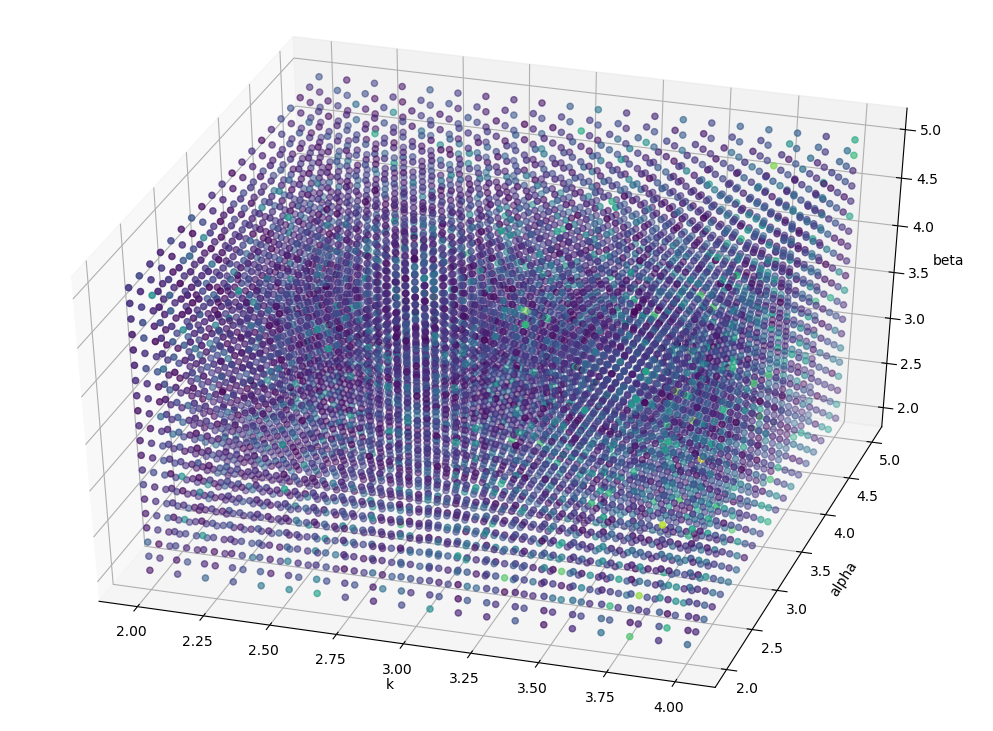
\includegraphics[width=0.8\textwidth]{./plots/ps_2N0M.png}
\caption[Parameter space search.]
{A search of a region of parameter space around $k$=3, $\alpha$=3,
$\beta$=3. The colour of each point represents a normalised scaling of
the sum of squared differences between elements of $c_0$ and $c_1$
after 5000 iterations of the simulation. The maximum value of this
metric was 0.0066; the minimum was 1.7 $\times$ 10$^{-5}$. For
comparison, the value of the metric for a guided system which
separated into two clear regions at 5000 steps was 722.}
\label{fig:ps_2N0M}
\end{figure}

I created two methods to run through the parameter space. One, called
\code{analysis/scanspace.py}, creates a json file for each parameter set, then
calls the program \code{james1c}, and finally
calls \code{sos\_centroid\_analyse()} to add each result
to \code{logs/scanspace.h5}. The problem with this method is that it
repeatedly creates the \code{morph::HexGrid}, adding lots of worthless
computation. To fix this, I wrote \code{ps\_2N0M.cpp}, which uses a
single \code{RD\_James} instance, which it re-sets after each
simulation, without having to re-compute the HexGrid. This can
evaluate 5000 timesteps of one parameter set with the Hex to Hex
spacing set to 0.02 in 1.3 seconds (on
threadbeast). \code{ps\_2N0M.cpp} runs the simulations, but it doesn't
apply the final analysis step of computing the sum of squared
differences between c0 and c1. This is carried out by
\code{analysis/ps\_2N0M\_postproc.py} and plotting by
\code{analysis/ps\_2N0M\_plot.py}. See Fig.~\ref{fig:ps_2N0M}.

\section{Two dimensional system with changed competition}

The symmetry of the terms for $\pm \alpha_i c_i$ and
$\pm \beta_i n a_i$ in
Equations \ref{eq:Karb1D_dc} \& \ref{eq:Karb1D_da} results directly
from the simple kinetic reaction:

\begin{equation} \label{eq:kinetic}
n + a_i \xrightleftharpoons[\alpha_{i}]{\beta_{i}} c_i
\end{equation}

If I want to change the competition between axons from different
thalamocortical regions, I need to consder exactly what it is about
Eq.~\ref{eq:kinetic} that I want to modify, so that the model is
changed with some sort of guiding principle.

Here are some modifications to the equations to enable competition
between regions dreamed up in just such a flagrant, un-principled way:

\subsection{Allow the branching rate of all other TC axon types to change $\dot{a}_i$}
%
\begin{equation} \label{eq:Karb2D_dc_compo_1}
\frac{\partial c_i(\mb{x},t)}{\partial t} = -\alpha_i c_i((\mb{x},t)
+ \beta_i n(\mb{x},t)
[a_i(\mb{x},t)]^k
\end{equation}
%
\begin{equation} \label{eq:Karb2D_da_compo_1}
\frac{\partial a_i(\mb{x},t)}{\partial t}
= \nabla\vcdot\mb{J}_i(\mb{x},t) + \alpha_i c_i(\mb{x},t) - \beta_i n(\mb{x},t)
[a_i(\mb{x}, t)]^k - \epsilon_i \sum_{j \ne i}^{N} a_j(\mb{x}, t)^l
\end{equation}
%
\begin{equation}
n(\mb{x},t) = 1 - \sum_{i=1}^{N} c_i(\mb{x}, t)
\end{equation}
%
with the flux current as given by Eq.~\ref{eq:Karb2D_J} and Neumann
boundary conditions as usual. This adds two parameter sets; $\epsilon$
and $l$.

See the binary \code{james1\_c1} for the implementation. Possibly
unstable; one TC type gets an initial advantage and this plays out
slowly (over fairly long timescale (10's of thousands of timesteps)
until one side wins.

The additional term could result from some sort of axon-axon repulsion
as the axons grow into the cortex, or an effect that occurs only once
they are growing within the cortical layer.

An implementation of this mechanism in \code{rd\_james\_comp1.cpp}
does not produce strong competition compared with the following
mechanism.

\subsection{Use \emph{all} the TC axon branching densities to contribute to flux current of axonal branching}

Change the flux current from:
%
\begin{equation} \label{eq:Karb2D_J_NM_again}
\mb{J}_i(\mb{x},t) = D \nabla a_i(\mb{x},t) - a_i
\sum_{j=1}^M \big(\gamma_{i,j} \nabla\rho_j(\mb{x}) \big)
\end{equation}
%
(which is a re-write of Eq.~\ref{eq:Karb2D_J_NM}) to:
%
\begin{equation} \label{eq:Karb2D_J_NM_with_comp}
\mb{J}_i(\mb{x},t) = D \nabla a_i(\mb{x},t)
- D' \nabla \textstyle \sum_{p\ne i}^N a_p(\mb{x},t) - a_i
\sum_{j=1}^M \big(\gamma_{i,j} \nabla\rho_j(\mb{x}) \big)
\end{equation}
%
or
%
\begin{equation} \label{eq:Karb2D_J_NM_with_comp2}
\mb{J}_i(\mb{x},t) = D \nabla \big(a_i(\mb{x},t) - \textstyle \sum_{p\ne i}^N a_p(\mb{x},t) \big) - a_i
\sum_{j=1}^M \big(\gamma_{i,j} \nabla\rho_j(\mb{x}) \big)
\end{equation}
%
which should be another way to add competition to the system. The idea
here is that branching density should flow away from regions where
there is a high level of branching of other TC axon types.

I settled on this implementation of
Eq.~\ref{eq:Karb2D_J_NM_with_comp2} in \code{rd\_james\_comp2.cpp}:
%
\begin{equation} \label{eq:Karb2D_J_NM_with_comp2_impl}
\mb{J}_i(\mb{x},t) = \nabla \big(D a_i(\mb{x},t) - \frac{D'}{N-1} \textstyle \sum_{p\ne i}^N a_p(\mb{x},t) \big) - a_i
\sum_{j=1}^M \big(\gamma_{i,j} \nabla\rho_j(\mb{x}) \big)
\end{equation}
%
which provides $D'$ as a parameter to define the strength of the
contribution of the non-self axon branching densities to the flux
current. The `positive' diffusion constant is $D$ (being positive,
this is kind of an \emph{infusion} constant), and the `negative'
diffusion is $\frac{D'}{N-1}$. This successfully produced competition
between $N$=2 TC types in the absence of any guidance molecules with
$D$=0.1 and $D'$ set to a value of 0.001.

\textbf{Stop press} Actually, no, this doesn't do anything interesting
at all, now that I've fixed the bugs. If $D=D'$ for a
\code{2N0M} system, then the system is static. If $D'$>$D$, then the
system is numerically unstable.

\subsection{Add an interaction with $\nabla n$}

Imagine that as connections are made to the cortical dendrites, a
molecule is expressed. Axon branching should expand into areas with
low connections, so the `flux of branching' should follow the gradient
of this `connectivity molecule' from high $n$ to low $n$. I've
expressed this by adding a new term to Eq.~\ref{eq:Karb2D_J_NM}:
%
\begin{equation} \label{eq:Karb2D_J_NM_with_comp3}
\mb{J}_i(\mb{x},t) = D \nabla a_i(\mb{x},t)
\boxed{-a_i(\mb{x}, t) D^n \nabla n(\mb{x}, t)}
 - a_i(\mb{x},t) \sum_{j=1}^M \big(\gamma_{i,j} \nabla\rho_j(\mb{x}) \big)
\end{equation}
%
With the new term (boxed), it's probably worth going back to look at the
method for computing $\nabla\vcdot\mb{J}_i$. Let's first write down that
%
\begin{equation} \label{eq:g_i}
\mb{g}_i(\mb{x}) = \sum_{j=1}^M \big(\gamma_{i,j} \nabla\rho_j(\mb{x}) \big)
\end{equation}
%
and then drop references to the space and time arguments ($\mb{g}_i(\mb{x})$
becomes $\mb{g}_i$; $n(\mb{x}, t)$ becomes $n$; and so on). This
allows a tidier version of Eq.~\ref{eq:Karb2D_J_NM_with_comp3} to be
written down:
%
\begin{equation} \label{eq:Karb2D_J_NM_with_comp3_simpler}
\mb{J}_i = D \nabla a_i - a_i D^n \nabla n - a_i \mb{g}_i
\end{equation}
%
The divergence of $\mb{J}_i$ is
%%%%
\begin{equation}
\begin{split}
\nabla\vcdot\mb{J}_i & = \nabla\vcdot \big[ D \nabla a_i - a_i
D^n \nabla n - a_i \mb{g}_i \big] \\
%
& =
D \dvrg a_i
- D^n \nabla\vcdot a_i \nabla n
- \nabla\vcdot a_i \mb{g}_i
\end{split}
\end{equation}
%
because the divergence operator is distributive (and $D$ \& $D^n$ are
scalar constants).  Applying the vector calculus product rule identity to
$\nabla\vcdot\big(a_i\nabla n\big)$ and
$\nabla\vcdot\big(a_i \mb{g}_i\big)$:
%
\begin{equation}
%
\nabla\vcdot\mb{J}_i = D \dvrg a_i
%
- D^n \big(
a_i \dvrg n + \nabla n \vcdot \nabla a_i
\big)
%
- \big(
a_i\nabla\vcdot\mb{g}_i
+
\mb{g}_i\vcdot\nabla a_i
\big)
%
\end{equation}
%
Expanding the brackets we have:
%
\begin{equation} \label{eq:divJExpanded2}
\boxed{
%
\nabla\vcdot\mb{J}_i = D \dvrg a_i
%
- D^n a_i \dvrg n
- D^n \nabla n \vcdot \nabla a_i
%
- a_i\nabla\vcdot\mb{g}_i
- \mb{g}_i\vcdot\nabla a_i
}
%
\end{equation}
%
which gives us 5 terms to compute in \code{compute\_divJ()} in place
of the original 3 terms in Eq.~\ref{eq:divJExpanded}.

\subsection{Initial conditions}

Initial reading of the literature suggests that axons grow towards
cortex in a `guideposted manner' and then start branching once within
the cortex. This would suggest that initial conditions should be more
targeted than in the Karbowski model, with axons of type $i$ arriving
in a region expected to be region $i$, but with the possibility of
modifying the model to simulate a denucleated animal by reducing the
density of incident visual TC axons, or reducing their branching rate.

I've implemented a scheme, using 2D Gaussians of varying (symmetrical)
width, gain and location, to make masks for the initial branching
densities for the different thalamocortical axon types.

\subsection{Agent based model}

It may be helpful to create a more realistic axon model, where axons
grow in a tree manner, with guidance and interactions, from physically
plausible locations in a virtual thalamus.

%
% BIBLIOGRAPHY
%
\selectlanguage{English}
\bibliographystyle{abbrvnotitle}
% The bibliography NoTremor.bib is the one exported from Zotero. It
% may be necessary to run my UTF-8 cleanup script, bbl_utf8_to_latex.sh
%%\bibliography{NoTremor}
%
% It produces this:
\begin{thebibliography}{1}

\bibitem{george_b._arfken_mathematical_1995}
{George B. Arfken} and H.~J. Weber.
\newblock {\em Mathematical {Methods} for {Physicists}}.
\newblock Academic Press, fourth edition edition, 1995.

\bibitem{karbowski_model_2004}
J.~Karbowski and G.~Ermentrout.
\newblock {\em Journal of Computational Neuroscience}, 17(3):347--363, Nov.
  2004.

\bibitem{lee_hexagonal_2014}
D.~Lee, H.~Tien, C.~Luo, et~al.
\newblock {\em International Journal of Computer Mathematics},
  91(9):1986--2009, Sept. 2014.

\end{thebibliography}

%%% Upload the *bib file along with the *tex file and PDF on
%%% submission if the bibliography is not in the main *tex file

\end{document}
